\section*{Anexo A. Tablas de eficiencias de ICB y esquemas de los modelo EI}
\addcontentsline{toc}{section}{Anexo A. Tablas de eficiencias de ICB y esquemas de los modelo EI}

\subsection*{A1. Eficiencia de los intervalos Bootstrap para el caso EI-NVC}
\addcontentsline{toc}{subsection}{A1. Eficiencia de los intervalos Bootstrap para el caso EI-NVC}

Con base en el promedio general (Figura \ref{fig:EficPromIntBootsTamMuestEsqRemuEI-NVC}) para: Eficiencia del ICB Percentil (Efic Int Boot Perc) y Eficiencia del ICB BCa (Efic Int Boot Bca) el mejor esquema resulto Liu2, 0.9627 y 0.9052 respectivamente;
Eficiencia del ICB Percentil cuando solo el lo contiene a la $R^{2}$ y Eficiencia del ICB BCa cuando solo el contiene a la $R^{2}$ el mejor esquema resulto Liu1, 0.5864 y 0.5751 respectivamente; 
la Eficiencia de ICB Percentil cuando gana en el empate a ICB BCa (Efic Boot Perc gana empate), el mejor esquema es Wu3 (0.3019) y la Eficiencia ICB BCa cuando gana en el empate al ICB Percentil (Efic Boot Bca gana empate), el mejor esquema es Wu2 (0.8626).\\


Sin considerar el tamaño de la muestra y esquema, para el caso EI-NVC los ICB mejores en promedio general (Figura \ref{fig:EficPromIntBootsTamMuestEsqRemuEI-NVC}) son: Eficiencia del ICB Percentil (Efic Int Boot Perc) con $0.8745$ ante la Eficiencia en ICB BCa (Efic Int Boot Bca); la Eficiencia del ICB Percentil cuando solo el contiene a la $R^{2}$ $(0.1413)$ y la Eficiencia de ICB BCa cuando gana en el empate al ICB Perc (Efic Boot Bca gana empate) con $0.7469$. Por lo que, el mejor es el ICB Percentil.


\begin{figure}[ht] 
	\centering 
	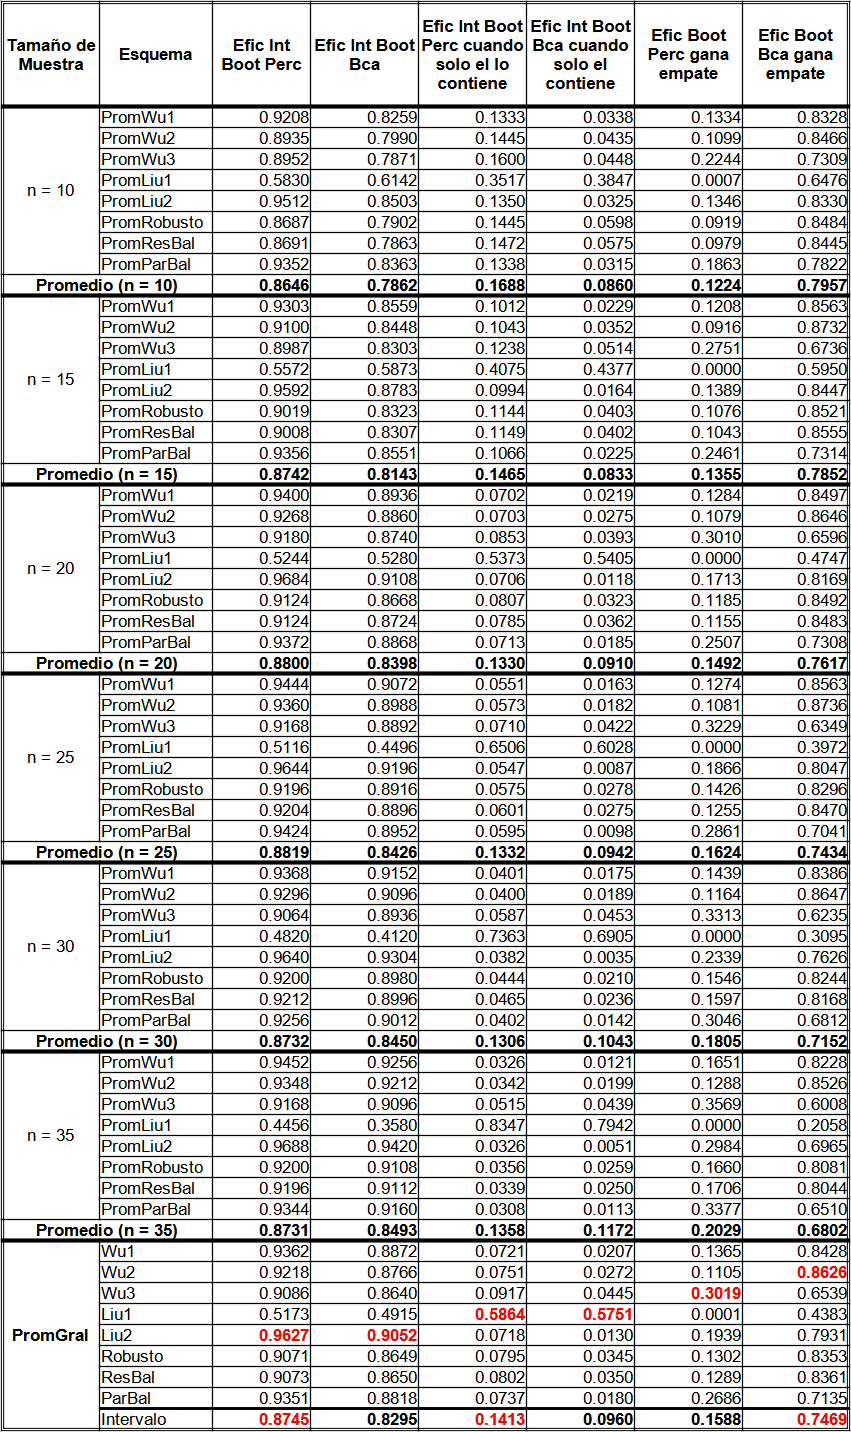
\includegraphics[width=0.55\linewidth]{img/EI_NVC_Efic_Boots.png} 
	\caption{Eficiencia promedio de los intervalos Bootstrap por tamaño de muestra y esquema de remuestreo para el caso EI-NVC.} 
	\label{fig:EficPromIntBootsTamMuestEsqRemuEI-NVC}
\end{figure}
\FloatBarrier



\subsection*{A2. Eficiencia de los esquemas para el caso EI-NVC}
\addcontentsline{toc}{subsection}{A2. Eficiencia de los esquemas para el caso EI-NVC}


Con base en al menos 90\% de eficiencia promedio y sin importar el ICB (Figura \ref{fig:EficPromEsqTamMuesEsqRemuEI-NVC}): con $n=10$ y $n=15$ ningún esquema cumplió la condición, sin embargo con ambos el mejor esquema es Liu2, con 0.8227 y 0.8639 respectivamente; con los tamaños de muestra 20, 25, 30 el mejor fue el esquema Lui2 y con el tamaño de muestra 35 los mejores esquemas fueron Wu1, Wu2, Liu2 y Pareado Balanceado (ParBal).\\

Sin considerar el tamaño de la muestra e ICB, para el caso EI-NVC el mejor promedio general (Figura \ref{fig:EficPromEsqTamMuesEsqRemuEI-NVC}) en eficiencia de esquema es Liu2 (0.8938).


\begin{figure}[ht] 
	\centering 
	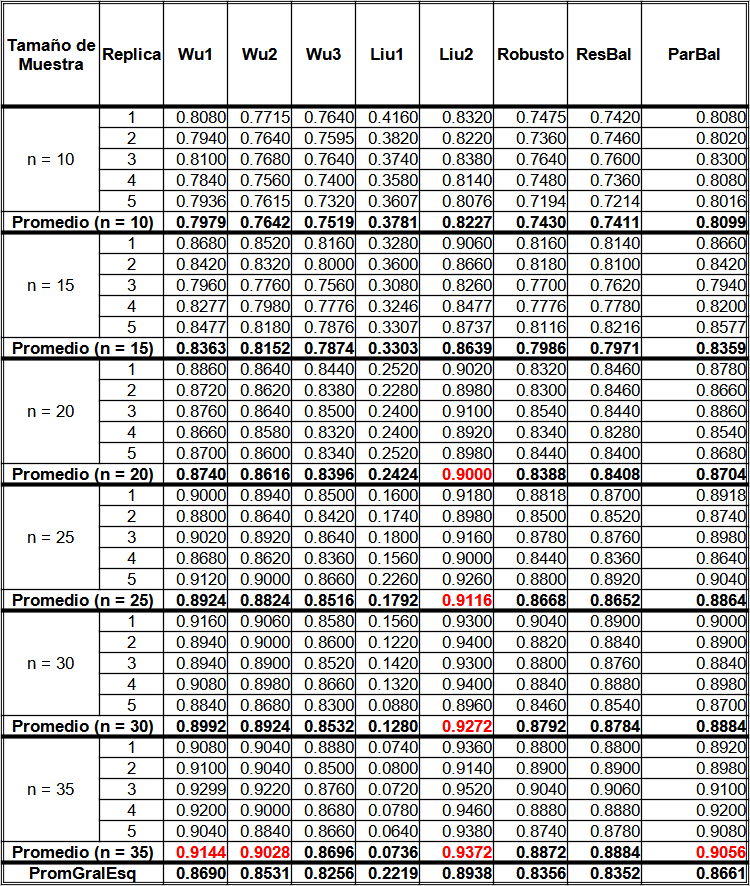
\includegraphics[width=0.70\linewidth]{img/EI_NVC_Efic_Esq.png} 
	\caption{Eficiencia promedio de los esquemas por tamaño de muestra para el caso EI-NVC.} 
	\label{fig:EficPromEsqTamMuesEsqRemuEI-NVC}
\end{figure}
\FloatBarrier

%%%%%%%%%%%%%%%%%%%%%%%%%%%%%%%%%%%%%%%%%%%%%%%%%%%%%%%%%%%%%
\subsection*{A3. Eficiencia de los intervalos Bootstrap para el caso EI-NNVC}
\addcontentsline{toc}{subsection}{A3. Eficiencia de los intervalos Bootstrap para el caso EI-NNVC}

Con base en el promedio general (Figura \ref{fig:EficPromIntBootsTamMuestEsqRemuEI-NNVC}) para: Eficiencia del ICB Percentil (Efic Int Boot Perc) y Eficiencia en ICB BCa (Efic Int Boot Bca) el mejor esquema resultó Liu2, 0.9603 y 0.9005 respectivamente;
Eficiencia del ICB Percentil cuando solo él contiene a la $R^{2}$ y Eficiencia del ICB BCa cuando solo él contiene a la $R^{2}$ el mejor esquema resultó Liu1, 0.5224 y 0.5304 respectivamente; la Eficiencia de ICB Percentil cuando gana en el empate a ICB BCa (Efic Boot Perc gana empate), el mejor esquema es Wu3 (0.6169) y la Eficiencia ICB BCa cuando gana el empate al ICB Percentil (Efic Boot Bca gana empate), el mejor esquema es Pareado Balanceado (ParBal) con 0.7493.\\

Sin considerar el tamaño de la muestra y esquema, para el caso EI-NNVC los ICB mejores en promedio general (Figura \ref{fig:EficPromIntBootsTamMuestEsqRemuEI-NNVC}) son: Eficiencia del ICB Percentil (Efic Int Boot Perc) con $0.8833$ ante la Eficiencia en ICB BCa (Efic Int Boot Bca); la Eficiencia del ICB Percentil cuando solo el contiene a la $R^{2}$ $(0.1467)$ y la Eficiencia de ICB BCa cuando gana en el empate al ICB Perc (Efic Boot Bca gana empate) con $0.6252$. Por lo que, el mejor ICB Percentil.


\begin{figure}[ht] 
	\centering 
	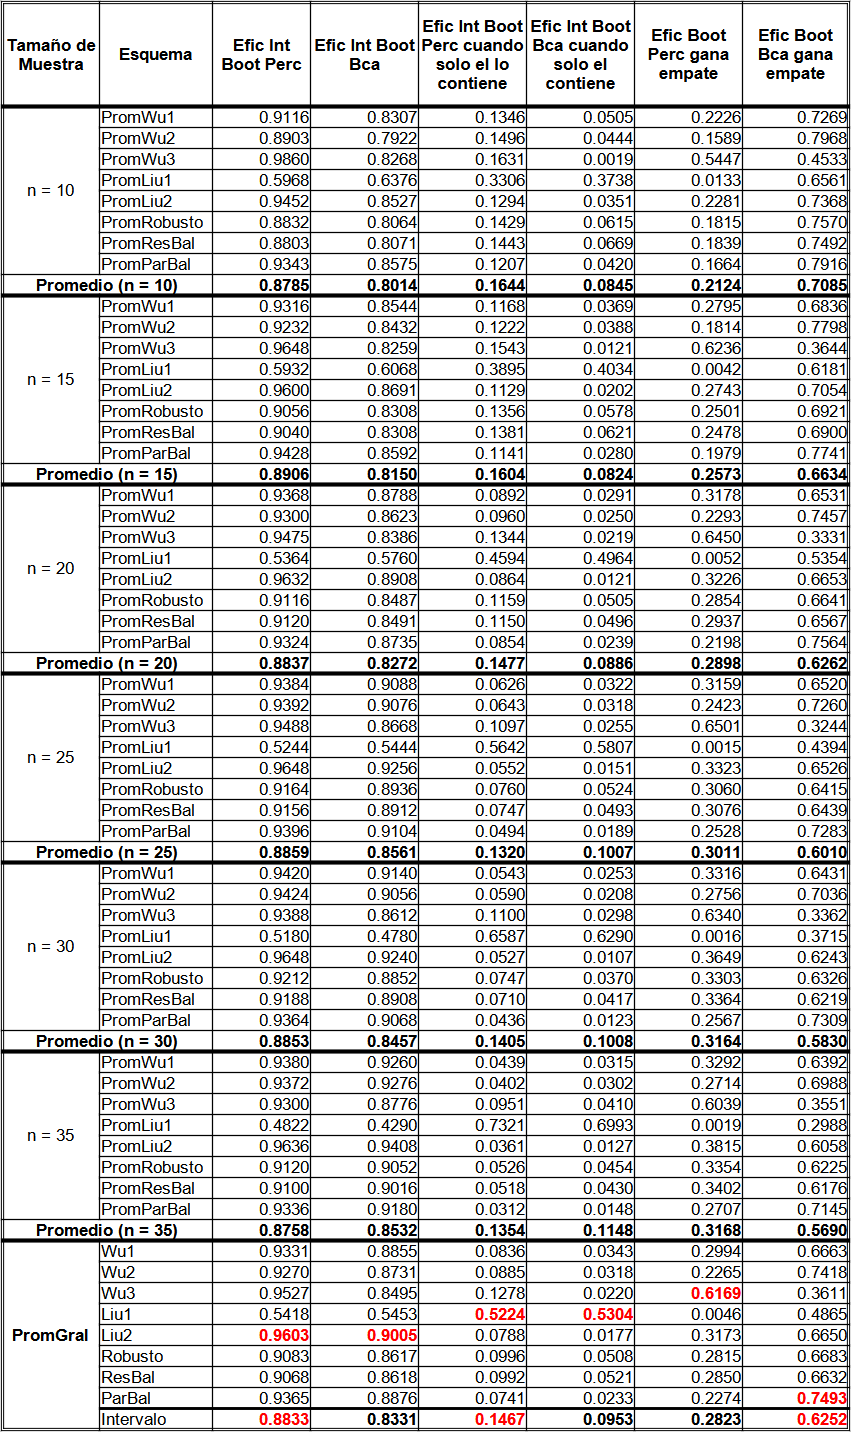
\includegraphics[width=0.55\linewidth]{img/EI_NNVC_Efic_Boots.png} 
	\caption{Eficiencia promedio de los intervalos Bootstrap por tamaño de muestra y esquema de remuestreo para el caso EI-NNVC.} 
	\label{fig:EficPromIntBootsTamMuestEsqRemuEI-NNVC}
\end{figure}
\FloatBarrier


\subsection*{A4. Eficiencia de los esquemas para el caso EI-NNVC}
\addcontentsline{toc}{subsection}{A4. Eficiencia de los esquemas para el caso EI-NNVC}


Con base en al menos 90\% de eficiencia promedio y sin importar el ICB (Figura \ref{fig:EficPromEsqTamMuesEsqRemuEI-NNVC}): con $n= 10, 15$ y $20$ ningún esquema cumplió la condición, sin embargo, al no considerar el criterio anterior, el mejor esquema para: n=10 es Wu3 (0.8252) y Liu2 (0.8215), n=15 es Liu2 (0.8515) y Pareado Balanceado (ParBar) con 0.8352 y n=20 es Liu2 (0.8800) y Wu1 (0.8532). Con el tamaño de muestra 25 el mejor esquema es Liu2 (0.9116) seguido por ParBal (0.8932), con tamaño de muestra 30 el mejor esquema es Liu2 (0.9140) seguido por ParBal (0.8956) y con el tamaño de muestra 35 los mejores esquemas son Liu2 y ParBal, con 0.9288 y 0.904 respectivamente.\\

Sin considerar el tamaño de la muestra e ICB, para el caso EI-NNVC los mejores promedios generales (Figura \ref{fig:EficPromEsqTamMuesEsqRemuEI-NNVC})  en eficiencia de esquema son Liu2 (0.8848) y ParBal (0.8671).

\begin{figure}[ht] 
	\centering 
	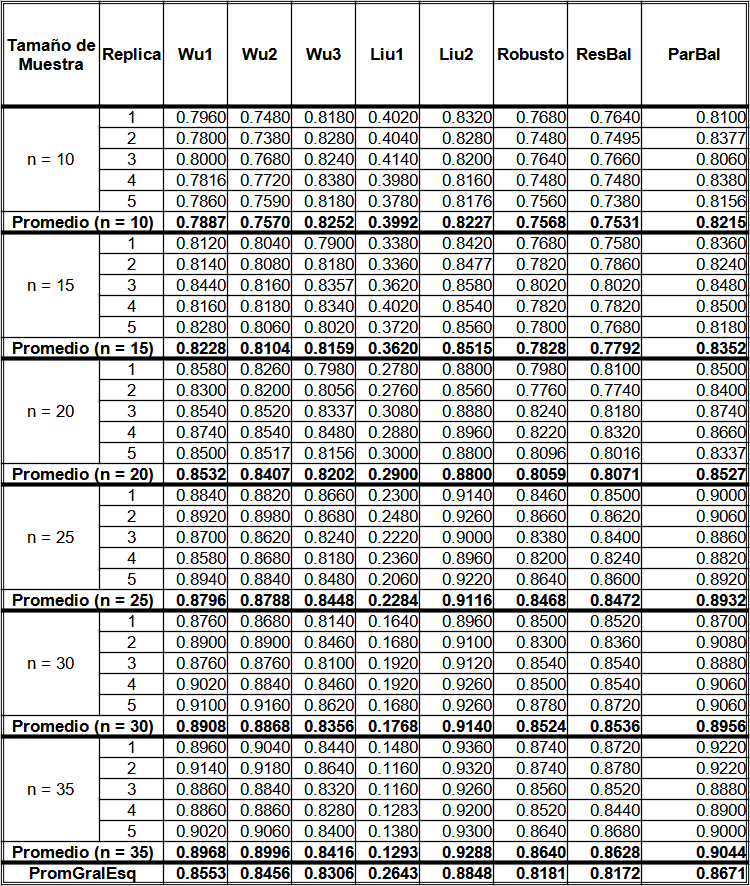
\includegraphics[width=0.70\linewidth]{img/EI_NNVC_Efic_Esq.png} 
	\caption{Eficiencia promedio de los esquemas por tamaño de muestra para el caso EI-NNVC.} 
	\label{fig:EficPromEsqTamMuesEsqRemuEI-NNVC}
\end{figure}
\FloatBarrier


%%%%%%%%%%%%%%%%%%%%%%%%%%%%%%%%%%%%%%%%%%%%%%%%%%%%%%%%%%%%%%%%%%%%
\subsection*{A5. Eficiencia de los intervalos Bootstrap para el caso EI-NVD}
\addcontentsline{toc}{subsection}{A5. Eficiencia de los intervalos Bootstrap para el caso EI-NVD}

Con base en el promedio general  (Figura \ref{fig:EficPromIntBootsTamMuestEsqRemuEI-NVD}) para: Eficiencia del ICB Percentil (Efic Int Boot Perc) el mejor esquema resultó Liu2 (0.9837), Eficiencia en ICB BCa (Efic Int Boot Bca) el mejor esquema resultó Pareado Balanceado(ParBal) con 0.8915; Eficiencia del ICB Percentil cuando solo él lo contiene a la $R^{2}$ y Eficiencia del ICB Bca cuando solo él contiene a la $R^{2}$ el mejor esquema resulto Liu1, 0.3799 y 0.3885 respectivamente; la Eficiencia de ICB Percentil cuando gana en el empate a ICB BCa (Efic Boot Perc gana empate), el mejor esquema es Residuales Balanceados(ResBal) con 0.3364 y la Eficiencia ICB BCa cuando gana el empate al ICB Percentil (Efic Boot Bca gana empate), el mejor esquema es Wu2 (0.7012).\\


Sin considerar el tamaño de la muestra y esquema, para el caso EI-NVD los ICB mejores en promedio general  (Figura \ref{fig:EficPromIntBootsTamMuestEsqRemuEI-NVD}) son: Eficiencia del ICB Percentil (Efic Int Boot Perc) con $0.9030$ ante la Eficiencia en ICB BCa (Efic Int Boot Bca); la Eficiencia del ICB Percentil cuando solo el contiene a la $R^{2}$ $(0.1402)$ y la Eficiencia de ICB BCa cuando gana en el empate al ICB Perc (Efic Boot Bca gana empate) con $0.6501$. Por lo que, el mejor es ICB Percentil

\begin{figure}[ht] 
	\centering 
	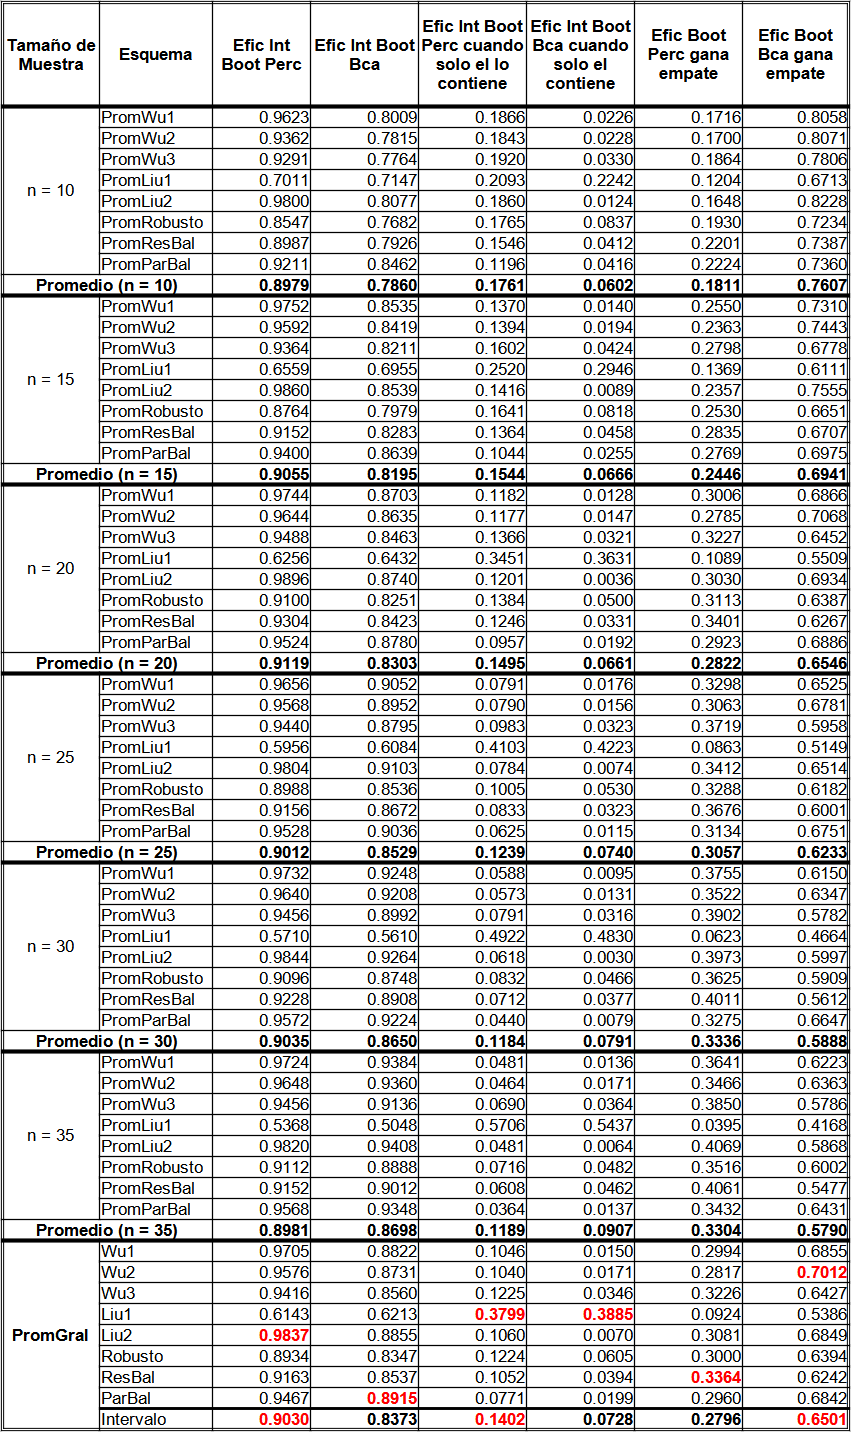
\includegraphics[width=0.55\linewidth]{img/EI_NVD_Efic_Boots.png} 
	\caption{Eficiencia promedio de los intervalos Bootstrap por tamaño de muestra y esquema de remuestreo para el caso EI-NVD.} 
	\label{fig:EficPromIntBootsTamMuestEsqRemuEI-NVD}
\end{figure}
\FloatBarrier

\subsection*{A6. Eficiencia de los esquemas para el caso EI-NVD}
\addcontentsline{toc}{subsection}{A6. Eficiencia de los esquemas para el caso EI-NVD}


Con base en al menos 90\% de eficiencia promedio y sin importar el ICB (Figura \ref{fig:EficPromEsqTamMuesEsqRemuEI-NVD}): con $n=10, 15$ y $20$ ningún esquema cumplió la condición,
sin embargo, al no considerar el criterio anterior, el mejor esquema para: n=10 es Pareado Balanceado (ParBal) con 0.8110, Liu2 (0.7977), Wu1 (0.7829) y Wu2 (0.7637); n=15 es Liu2 (0.8463), ParBal (0.8419), Wu1 (0.8415) y Wu2 (0.8255), y n=20 Liu2 (0.8708), ParBal (0.8612), Wu1 (0.8591) y Wu2 (0.7637). Con el tamaño de muestra 25 el mejor esquema es Liu2 (0.9035) seguido por ParBal (0.8932), Wu1 (0.8892) y Wu2 (0.881); con tamaño de muestra 30 los mejores esquemas son Liu2 (0.9236),  Wu1 (0.9160), ParBal (0.9152) y Wu2 (0.9088), y con el tamaño de muestra 35 los mejores esquemas son Liu2 (0.9348),  Wu1 (0.9256), ParBal (0.922) y Wu2 (0.92).\\

Sin considerar el tamaño de la muestra, para el caso EI-NVD el mejor promedio general (Figura \ref{fig:EficPromEsqTamMuesEsqRemuEI-NVD}) en eficiencia de esquema son Liu2 (0.8794), ParBal (0.8741), Wu1 (0.8690) y Wu2 (0.8583).

\begin{figure}[ht] 
	\centering 
	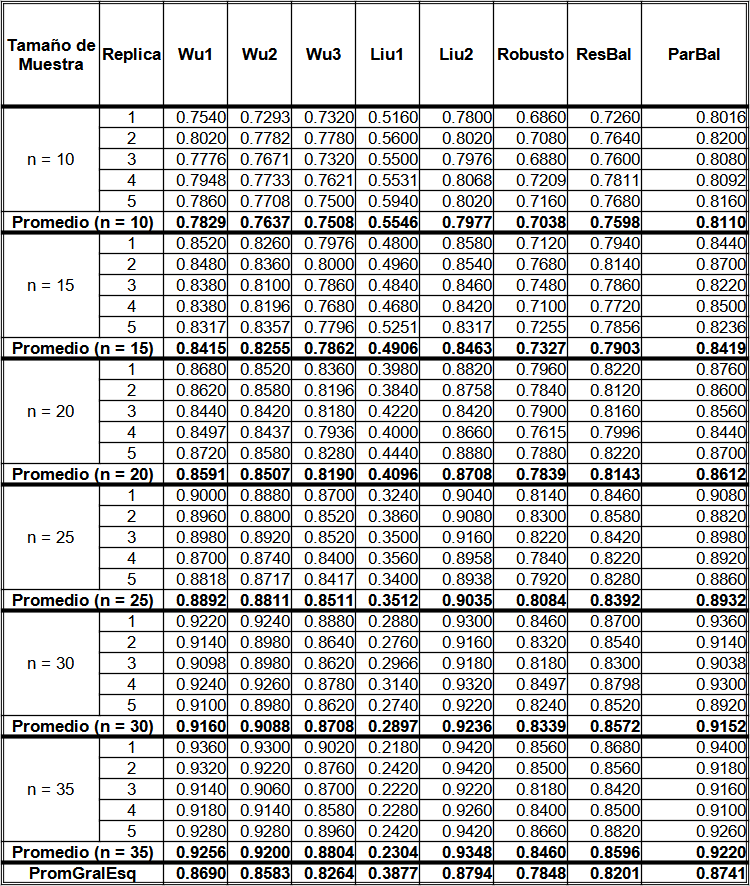
\includegraphics[width=0.70\linewidth]{img/EI_NVD_Efic_Esq.png} 
	\caption{Eficiencia promedio de los esquemas por tamaño de muestra para el caso EI-NVD.} 
	\label{fig:EficPromEsqTamMuesEsqRemuEI-NVD}
\end{figure}
\FloatBarrier



%%%%%%%%%%%%%%%%%%%%%%%%%%%%%%%%%%%%%%%%%%%%%%%%%%%%%%%%%%

\subsection*{A7. Eficiencia de los intervalos Bootstrap para el caso EI-NNVD}
\addcontentsline{toc}{subsection}{A7. Eficiencia de los intervalos Bootstrap para el caso EI-NNVD}

Con base en el promedio general (Figura \ref{fig:EficPromIntBootsTamMuestEsqRemuEI-NNVD}) para: Eficiencia del ICB Percentil (Efic Int Boot Perc) el mejor esquema resultó Liu2 (0.9554), Eficiencia en ICB BCa (Efic Int Boot Bca) el mejor esquema resultó Pareado Balanceado (ParBal) con 0.8882; Eficiencia del ICB Percentil cuando solo él lo contiene a la $R^{2}$ el mejor esquema resulto Wu3 (0.2807), Eficiencia del ICB BCa cuando solo él contiene a la $R^{2}$ el mejor esquema resultó Liu1 (0.1632); la Eficiencia de ICB Percentil cuando gana en el empate a ICB BCa (Efic Boot Perc gana empate), el mejor esquema es Residuales Balanceados(ResBal) con 0.5197 y la Eficiencia ICB BCa cuando gana el empate al ICB Percentil (Efic Boot Bca gana empate), el mejor esquema es ParBal (0.5074).\\

Sin considerar el tamaño de la muestra y esquema, para el caso EI-NNVD los ICB mejores en promedio general (Figura \ref{fig:EficPromIntBootsTamMuestEsqRemuEI-NNVD}) son: Eficiencia del ICB Percentil (Efic Int Boot Perc) con $0.9035$ ante la Eficiencia en ICB BCa (Efic Int Boot Bca); la Eficiencia del ICB Percentil cuando solo el contiene a la $R^{2}$ $(0.1940)$ y la Eficiencia de ICB BCa cuando gana en el empate al ICB Perc (Efic Boot Bca gana empate) con $0.5074$.Por lo que, el mejor es ICB Percentil.

\begin{figure}[ht] 
	\centering 
	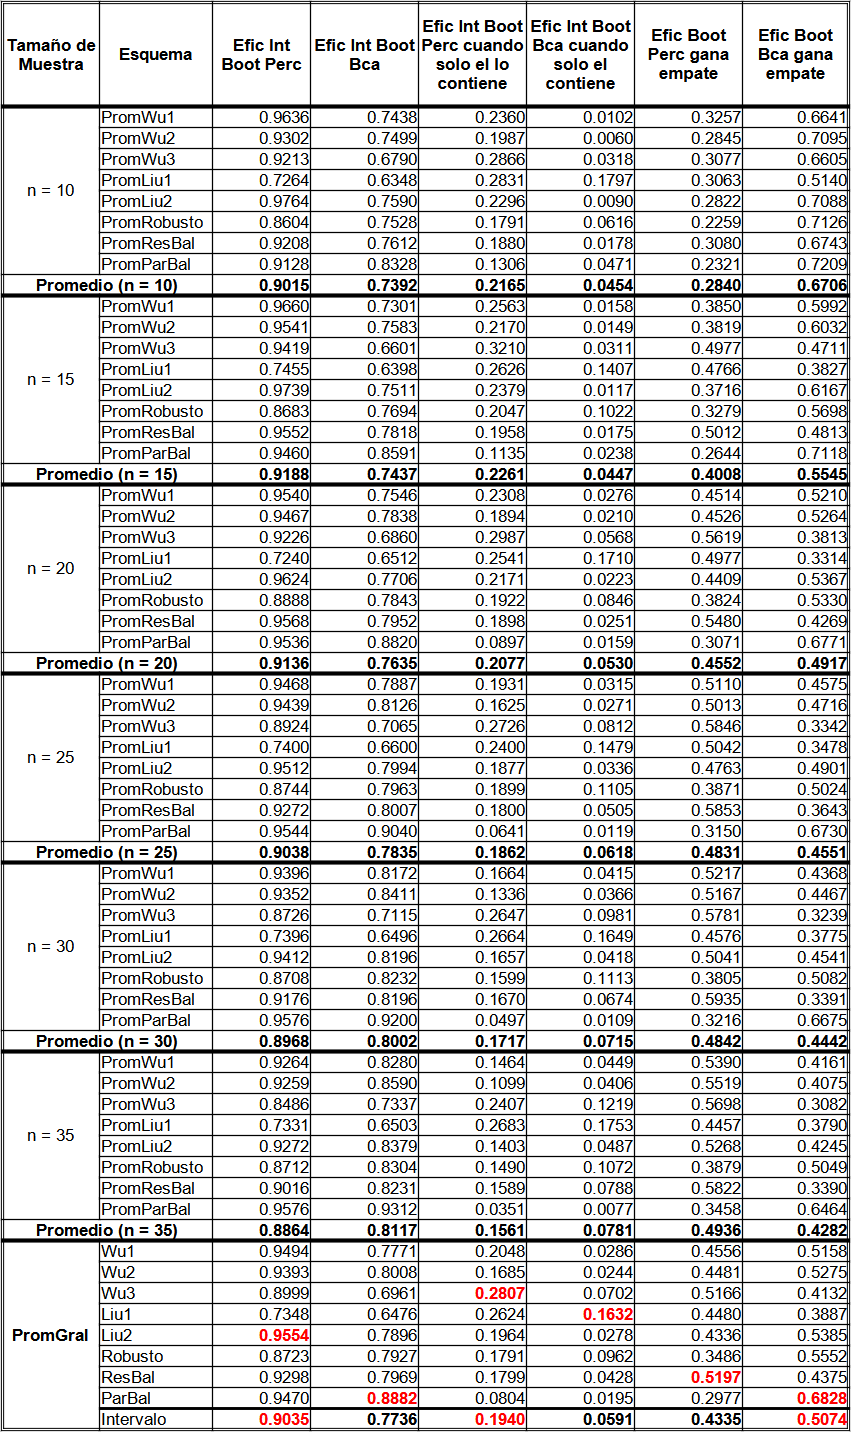
\includegraphics[width=0.55\linewidth]{img/EI_NNVD_Efic_Boots.png} 
	\caption{Eficiencia promedio de los intervalos Bootstrap por tamaño de muestra y esquema de remuestreo para el caso EI-NNVD.} 
	\label{fig:EficPromIntBootsTamMuestEsqRemuEI-NNVD}
\end{figure}
\FloatBarrier


\subsection*{A8. Eficiencia de los esquemas para el caso EI-NNVD}
\addcontentsline{toc}{subsection}{A8. Eficiencia de los esquemas para el caso EI-NNVD}

Con base en al menos 90\% de eficiencia promedio y sin importar el ICB (Figura \ref{fig:EficPromEsqTamMuesEsqRemuEI-NNVD}): con $n=10, 15, 20$ y $25$ ningún esquema cumplió la condición, sin embargo, al no considerar el criterio anterior, el mejor esquema para: n=10 es Pareado Balanceado (ParBal) con 0.7936; $n=15$ es (ParBal) con 0.8387;  n=20 es ParBal (0.8680) y  n=25 es ParBal (0.8932). Con los tamaños de muestra 30 y 35 el mejor esquema es ParBal, 0.91 y 0.9240 respectivamente.\\

Sin considerar el tamaño de la muestra, para el caso EI-NNVD el mejor promedio general (Figura \ref{fig:EficPromEsqTamMuesEsqRemuEI-NNVD}) en eficiencia de esquema es ParBal (0.8713).


\begin{figure}[ht] 
	\centering 
	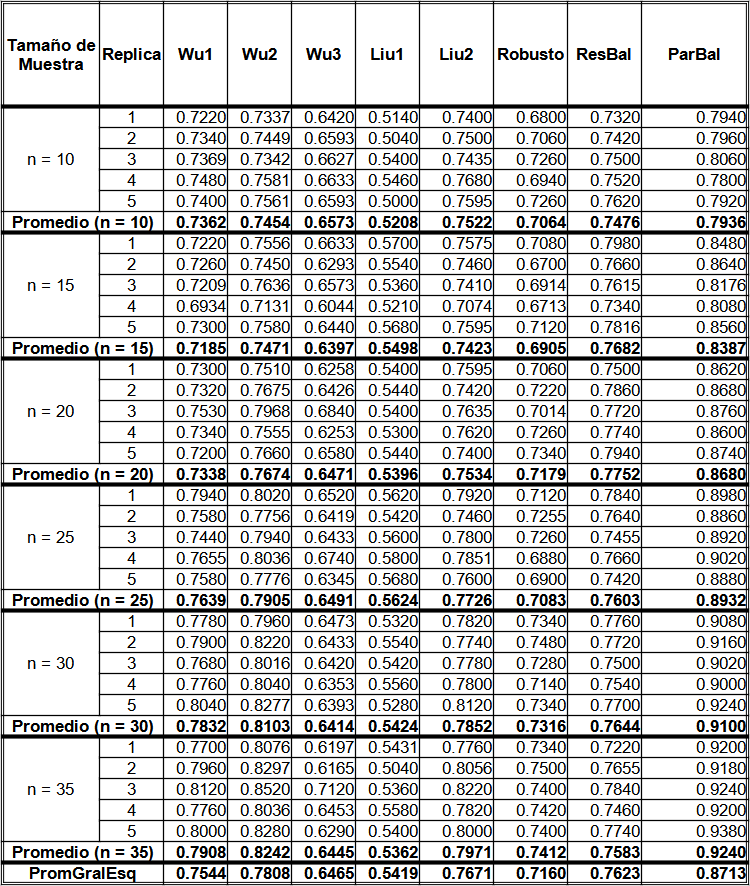
\includegraphics[width=0.70\linewidth]{img/EI_NNVD_Efic_Esq.png} 
	\caption{Eficiencia promedio de los esquemas por tamaño de muestra para el caso EI-NNVD.} 
	\label{fig:EficPromEsqTamMuesEsqRemuEI-NNVD}
\end{figure}
\FloatBarrier

%%%%%%%%%%%%%%%%%%%%%%%%%%%%%%%%%%%%%%%%%%%%%%%%%%%%%%%%%%%%%
\clearpage
